\documentclass{beamer}

\usepackage[spanish]{babel}
\selectlanguage{spanish}
\usepackage[utf8]{inputenc}
\setbeamersize{text margin left=10mm,text margin right=1mm}

\title % (optional, only for long titles)
{TypeScript}
\author[Author, Anders] % (optional, for multiple authors)
{Sergio Álvarez Alonso \\ Adrián Mínguez Graña \\  Mario Moraño Orviz \\ 
Ángel Manuel Méndez Campal}
\institute[Universities Here and There] % (optional)
{
	\inst{}%
	Máster ingeniería web\\
	Universidad de Oviedo

}
\date[KPT 2004] % (optional)
{Diciembre 2018}
\subject{Computer Science}

\begin{document}
	
	\frame{\titlepage}
	
\small
\begin{frame}{Contexto y motivación del lenguaje I}
\begin{columns}[T] % contents are top vertically aligned
	\begin{column}[T]{8cm} % each column can also be its own environment

		\begin{itemize}
			\item Lanzado primera vez en 2012 (versión 0.8)
			\item 2 años de desarrollo interno en Microsoft
			\item Limitaciones de js para desarrollos de gran escala
			\item ``Adelanto'' de lo que cabría esperar de ECMAScript2015
			\item Anders Hejlsberg (LA de C\#) involucrado en el desarrollo
			\item Se transcompila a javascript
			\item Licencia Apache 2 (open source)
			\item Versión estable 3.1.6, 1 Noviembre
		\end{itemize}
	
	\end{column}
	\begin{column}[T]{3cm} % alternative top-align that's better for graphics
		
\includegraphics[height=3cm]{../imagenes/ts.png}
		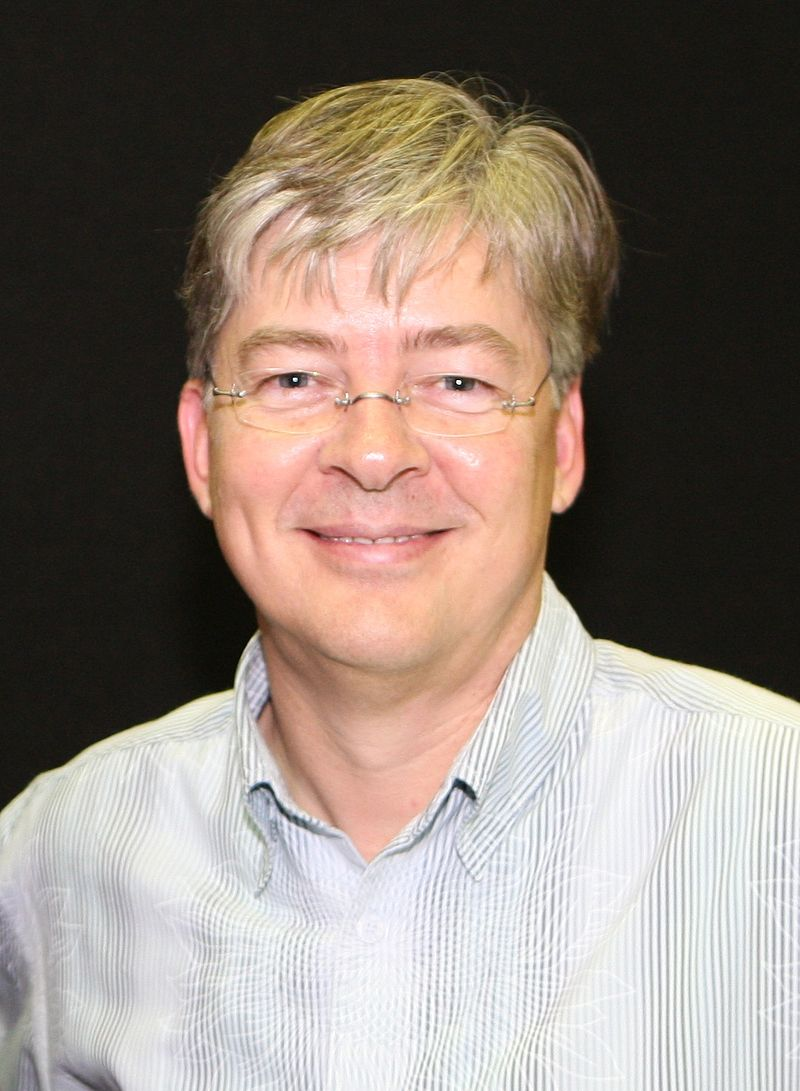
\includegraphics[height=3cm]{../imagenes/anders.jpg}
	\end{column}

\end{columns}

\begin{block}{Herramientas}
	Al principio sólo Visual Studio. Luego Eclipse, Emacs, Vim, Sublime, Webstorm,
	Atom y Visual Studio Code.
\end{block}

\end{frame}


\begin{frame}{Contexto y motivación del lenguaje II}
\begin{columns}[T] % contents are top vertically aligned
	\begin{column}[T]{7cm} % each column can also be its own environment
		Objetivos:
		\begin{itemize}
			\item Dotar js con un sistema opcional de tipos
			\item Proveer a los motores de js actuales de características planeadas para versiones futuras
		\end{itemize}
		Superset de javascript: .js $\to$ .ts y compilar devuelve js válido \\
		
		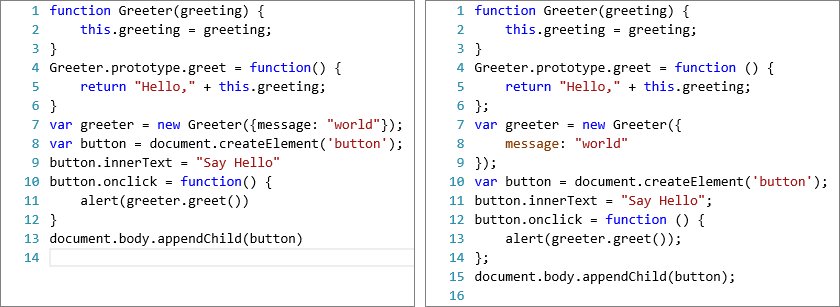
\includegraphics[height=3cm]{../imagenes/ts3.png}
	
		
	\end{column}
	\begin{column}[T]{3cm} % alternative top-align that's better for graphics
		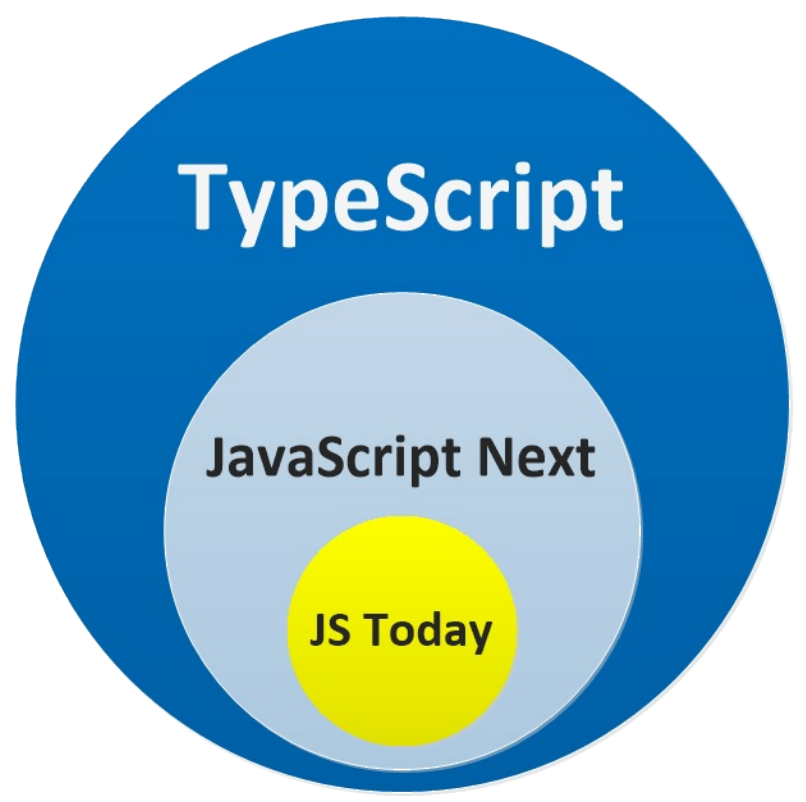
\includegraphics[height=3cm]{../imagenes/ts2.png}
		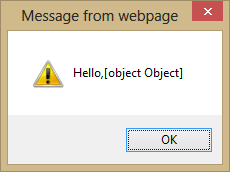
\includegraphics[height=3cm]{../imagenes/ts4.png}
	\end{column}
\end{columns}

\end{frame}

\small
\begin{frame}{Contexto y motivación del lenguaje III}
\begin{columns}[t, onlytextwidth]
	\begin{column}[T]{.6\textwidth} % each column can also be its own environment
		
		Añade anotación de tipos que se borra al transcopilar\\
		Más información en tiempo de compilación \\
		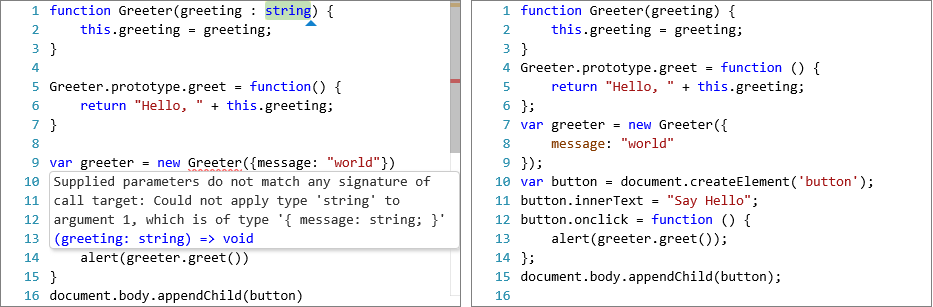
\includegraphics[height=2.5cm]{../imagenes/ts5.png}
		
		Declaración de clases y modularidad \\
		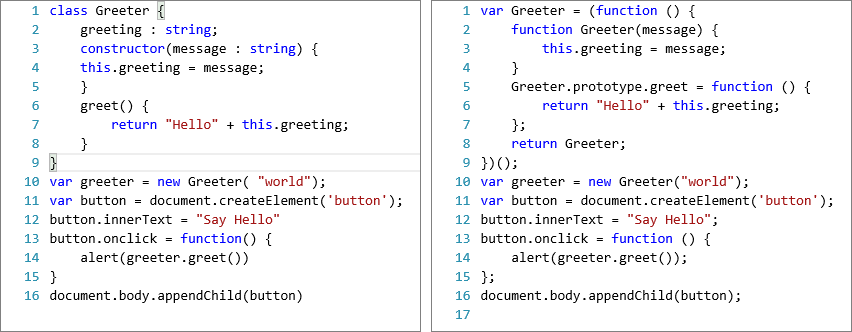
\includegraphics[height=2.5cm]{../imagenes/ts7.png}
		
		
	\end{column}
	\begin{column}[T]{0.3\textwidth} % alternative top-align that's better for graphics
		IntelliSense
		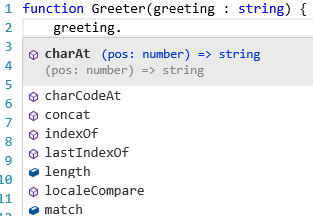
\includegraphics[height=2cm]{../imagenes/ts6.png} \\ 
		\hfill \break
		\\
		
		Sintaxis de declaración de tipos de ECS6 \\
		Produce código js preparado para hacer
		herencia por prototipos \\
		
		
\includegraphics[height=2cm]{../imagenes/ts8.png}
	
	\end{column}
\end{columns}
Escalar sitios web a aplicaciones más grandes

\end{frame}




\small
\begin{frame}{Referencias}
\begin{itemize}  
	\item https://blogs.msdn.microsoft.com/somasegar/2012/10/01 \\ /typescript-javascript-development-at-application-scale/
	\item The second item 
	\item The third etc \ldots 
\end{itemize}

\end{frame}

  \begin{frame}
\frametitle{Principales características}
In progress...
\end{frame}

\begin{frame}
\frametitle{Ejemplo de aplicación}
In progres...
\end{frame}

\begin{frame}
\frametitle{Valoración del lenguaje}
In progres...
\end{frame}


\end{document}